% !TeX spellcheck = cs_CZ
{\tikzset{external/prefix={tikz/FYZI/}}
 \tikzset{external/figure name/.add={ch27_}{}}
%---------------------------------------------------------------------------------------------------
% file fey1ch27.tex
%---------------------------------------------------------------------------------------------------
%========================= Geometrická optika ======================================================
\chapter{Geometrická optika}\label{fyz:IchapXXVII}
\minitoc

  \section{Úvod}\label{fyz:IchapXXVIIsecI}
    Na několika přístrojích předvedeme aproximaci nazvanou \emph{geometrická optika}. Je to
    nejužitečnější aproximace pro praktickou konstrukci mnoha optických systémů a přístrojů.
    Geometrická optika je buď velmi jednoduchá nebo velmi komplikovaná.
    
    Abychom mohli pokračovat potřebujeme jeden geometrický vztah a to: máme-li trojúhelník s malou
    výškou $h$ a velkou základnou $d$, pak přepona $s$ je delší než základna (viz obr.
    \ref{fyz:fig156}).  
    
    Tedy 
    \begin{equation}\label{FYZ:eq_triangle}
     \Delta \approx \frac{h^2}{2s}.
    \end{equation}
    To je celá geometrie, kterou je třeba znát, aby bylo možné diskutovat vznik obrazů pomocí
    zakřivených ploch.
    
    \begin{figure}[ht!] %\ref{fyz:fig156}
      \centering
      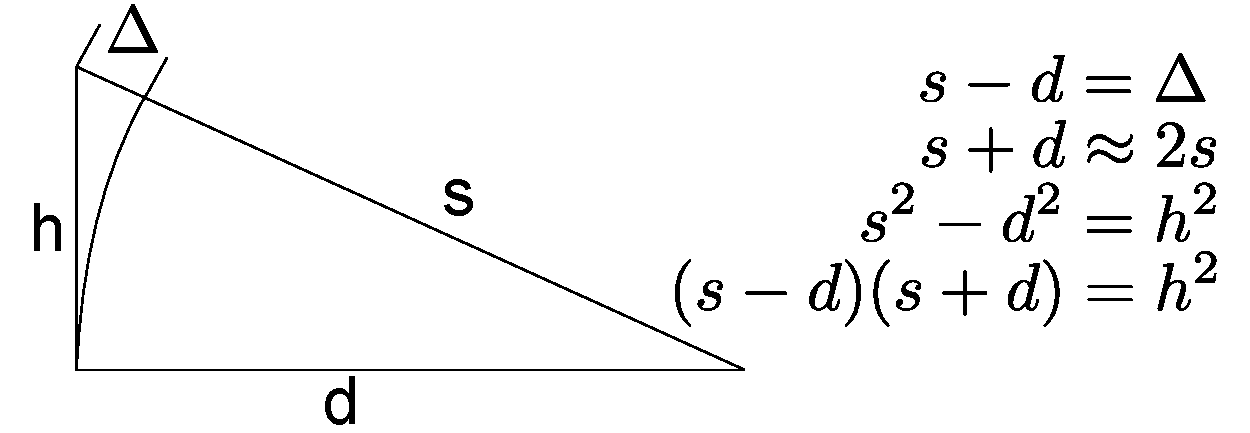
\includegraphics[width=0.6\linewidth]{fyz_fig156.pdf}
      \caption{Trojúhelník s malou výškou a velkou základnou
               \cite[s.~358]{Feynman01}}
      \label{fyz:fig156}  
    \end{figure}

  \section{Ohnisková vzdálenost kulové čočky}\label{fyz:IchapXXVIIsecII}
    První a nejjednodušší situace pro diskuzi je jediná plocha oddělující dvě prostředí s různými 
    indexy lomu (obr. \ref{fyz:fig303}). Případem libovolných indexů se nyní zabývat nebudeme, 
    neboť důležitější jsou vždy ideje, než určité konkrétní situace, a tento příklad je dost 
    jednoduchý, aby ho bylo možné vyřešit v kterémkoliv případě. Budeme předpokládat, že nalevo od 
    plochy je rychlost světla rovna \num{1} a napravo \(1/n\), kde \(n\) je \emph{index lomu}. Ve 
    skle se světlo šíří \(n\)-krát pomaleji.

    \begin{figure}[ht!] %\ref{fyz:fig303}
      \centering
      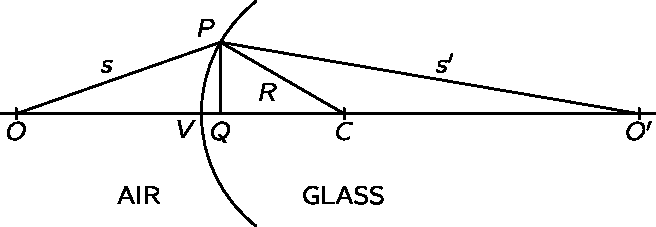
\includegraphics[width=0.6\linewidth]{fyz_fig303.pdf}
      \caption{Zaostření jedinou lámavou plochou
               \cite[s.~358]{Feynman01}}
      \label{fyz:fig303}  
    \end{figure}
    
    Nyní předpokládejme, že ve vzdálenosti \(s\) od nějakého bodu na povrchu skla máme bod \(O\) a 
    ve vzdálenosti \(s'\) máme jiný bod \(0'\) uvnitř skla a že zakřivený povrch skla chceme 
    upravit tak, aby každý paprsek vycházející z \(O\), jenž dopadne na povrch skla v kterémkoli 
    bodě \(P\) se lomil tak, že bude pokračovat do bodu \(O'\). Proto musíme dát povrchu takový 
    tvar, aby se doba, za niž projde paprsek zbodu \(O\) do bodu \(P\), tj. vzdálenost \(OP\) 
    dělená rychlostí světla (zde je jeho rychlost rovna jedné) plus \(n\)-krát \(O'P\), což je 
    doba, za niž projde z \(P\) do \(O'\), rovnala konstantě nezávislé na poloze \(P\). Z této 
    podmínky dostaneme rovnici k určení tvaru povrchu. Výsledek je takový, že povrch je dán velmi 
    komplikovanou křivkou čtvrtého stupně a může se bavit pokusem vypočítat ji pomocí analytické 
    geometrie. Jednodušší je pokusit se ji vypočítat pro zvláštní případ, kdy 
    \(s\rightarrow\infty\), neboť tehdy je to křivka druhého stupně a lze ji snadněji poznat. 
    Zajímavé je porovnání této křivky s \emph{parabolou}, kterou jsme našli pro zrcadlo 
    soustředující paprsky přicházející znekonečna do jednoho bodu.
    
    Takže přiměřený povrch nelze snadno připravit - soustředit světlo vycházející z jednoho bodu v 
    jiném bodě vyžaduje dost komplikovanou plochu. V praxi se obvykle nesnažíme vytvořit tak 
    komplikované povrchy, ale děláme kompromis. Místo toho, abychom se snažili dostat do ohniska 
    všechny paprsky, provádíme to tak, že do ohniska jdou pouze paprsky dost blízké k ose \(00'\). 
    Vzdálenější paprsky se mohou odchylovat, chtějí-li, neboť ideální povrch je složitý a místo něj 
    používáme kulovou plochu se správným poloměrem křivosti na ose. Výroba kulové plochy je mnohem 
    snadnější než výroba jiných povrchů, proto je pro nás užitečné, abychom zjistili, co se stane s 
    paprsky dopadajícími na kulový povrch za předpokladu, že pouze paprsky dostatečně blízké k ose 
    budou přesně soustředěny do ohniska. Paprsky \emph{blízké} ose se někdy nazývají 
    \textbf{paraxiální paprsky} a to, co analyzujeme, jsou podmínky k soustředění paraxiálních 
    paprsků do ohniska. Diskuzi o chybách, jež vznikají proto, že ne všechny paprsky jsou vždy 
    blízko osy, provedeme později.
    
    Za předpokladu, že \(P\) se nachází blízko osy, spustíme kolmici \(PQ\) tak, aby byla výška 
    \(PQ\) rovna \(h\). Na okamžik si představme, že povrch skla tvoří rovinu procházející bodem 
    \(P\). V takovém případě by čas potřebný na cestu z bodu \(O\) do \(P\) byl delší než čas z 
    \(O\) do \(Q\), a také čas z \(P\) do \(0'\) by byl delší než čas z \(Q\) do \(O'\). Ale to je 
    právě důvod, proč musí být povrch skla zakřiven, neboť celkový nadbytečný čas se musí 
    vykompenzovat zpožděním světla při cestě z \(V\) do \(Q\). Nadbytečný čas po dráze \(OP\) je 
    roven \(h^2/2s\) a nadbytečný čas po další části dráhy je roven \(h^2/2s'\). Tento nadbytečný 
    čas, jenž se musí přizpůsobit zpoždění podél dráhy \(VQ\), se liší od času, jenž by platil pro 
    vakuum, neboť je zde jiné optické prostředí. Jinými slovy, čas, který světlo potřebuje na cestu 
    z \(V\) do \(Q\), je jiný v tomto prostředí než ve vzduchu, světlo je pomalejší o faktor \(n\), 
    takže zpoždění na této vzdálenosti je pak \((n-1)VQ\). Otázkou je, jak velké je \(VQ\). Je-li 
    střed koule v bodě \(C\) a její poloměr je \(R\), vidíme, na základě téhož vzorce, že 
    vzdálenost \(VQ\) je rovna \(h^2/2R\). Tak jsme objevili zákon dávající do souvislosti 
    vzdálenosti \(s\) a \(s'\), jenž určuje hledaný poloměr křivosti \(R\). Tento zákon je
    \begin{subequations}\label{fyz:eq360}
      \begin{align}
        \frac{h^2}{2s} + n\frac{h^2}{2s'} &= (n-1)\frac{h^2}{2R} \label{fyz:eq360a} \\
        \shortintertext{neboli}
        \frac{1}{s} + n\frac{1}{s'}       &= \frac{n-1}{R}.      \label{fyz:eq360b}
      \end{align}    
    \end{subequations}

    Je-li dána poloha bodu \(O\) a druhého bodu \(O'\) a chceme světlo z \(O\) soustředit do 
    \(O'\), můžeme si požadovaný poloměr křivosti povrchu pomocí tohoto vzorce vypočítat.
    
    Z toho vidíme také zajímavý fakt, že stejná čočka se stejným poloměrem křivosti \(R\) bude 
    soustřeďovat paprsky i pro jiné vzdálenosti, konkrétně, pro jakýkoliv pár vzdáleností, pro něž 
    platí, že součet jejich převrácených hodnot, z nichž jedna je vynásobena \(n\), je rovna 
    konstantě. Takže daná čočka (omezíme-li se na paraxiální paprsky) bude soustřeďovat paprsky 
    nejen z bodu \(O\) do \(O'\), ale pro nekonečně mnoho jiných párů bodů, platí-li pro tyto páry 
    vztah, že \(\frac{1}{s} + \frac{n}{s'}\) je rovno konstantě charakteristické pro danou čočku.
    
    Zvláštní zajímavý případ je pro \(s\rightarrow\infty\). Ze vztahu je vidět, že když se jedno 
    \(s\) zvětšuje, druhé se zmenšuje. Jinak řečeno, vzdaluje-li se bod \(O\) do nekonečna, bod 
    \(0'\) se pohybuje uvnitř materiálu, dokud nedosáhne určité vzdálenosti, nazvané 
    \textbf{ohnisková vzdálenost} \(f'\). Přicházející rovnoběžné paprsky protnou osu ve 
    vzdálenosti \(f'\). Podobný proces si můžeme představit i z druhé strany. (Pamatujme na 
    pravidlo reciprocity: Půjde-li světlo z bodu \(O\) do \(O'\), půjde také z \(O'\) do \(O\)) 
    Kdyby byl zdroj světla uvnitř skla, mohli bychom se ptát, kde bude ohnisko. Ve zvláštním 
    případě, bude-li zdroj světla ve skle nekonečně daleko (týž problém), kde by se na venkovní 
    straně světlo soustředilo? Tato vzdálenost se nazývá \(f\). Samozřejmě můžeme se na věc dívat i 
    opačně. Kdyby byl zdroj světla ve vzdálenosti \(f\) a světlo by proniklo povrchem skla, šířilo 
    by se dál jako rovnoběžný svazek. Hodnoty \(f\) a \(f'\) můžeme snadno najít:
    \begin{subequations}\label{fyz:eq361}
      \begin{align}
        \frac{n}{f'}&=\frac{n-1}{R} \quad\text{neboli}\quad f'=\frac{Rn}{n-1}, \label{fyz:eq361a} \\
        \frac{1}{f} &=\frac{n-1}{R} \quad\text{neboli}\quad f=\frac{R}{n-1}, \label{fyz:eq361b} 
      \end{align}
    \end{subequations}

    Vidíme zajímavou věc: Vydělíme-li každou ohniskovou vzdálenost příslušným indexem lomu, 
    dostaneme stejný výsledek! Tento teorém je skutečně obecný. Platí pro jakýkoliv systém čoček, 
    bez ohledu na to, jak je komplikovaný, takže stojí za to si jej zapamatovat. Zde jsme 
    nedokázali jeho obecnost -jen jsme si všimli, že platí projediný povrch. Ukazuje se však, že 
    obecně platí, že dvě ohniskové vzdálenosti nějakého systému takto navzájem souvisí. Rovnice 
    (\ref{fyz:eq360}) se někdy píše ve tvaru
    \begin{equation}\label{fyz:eq362}
        \frac{1}{s} + \frac{n}{s'} = \frac{1}{f}.
    \end{equation}
    To je užitečnější vztah než vztah (\ref{fyz:eq360}), neboť \(f\) můžeme změřit mnohem snadněji 
    než poloměr křivosti a index lomu čočky. Nezajímáme-li se o to, jak zkonstruovat čočku, nebo o 
    to, jak byla zkonstruována, ale prostě ji sundáme z poličky a použijeme, pak je pro nás 
    zajímavé pouze \(f\) a nikoli \(n\), nebo \(R\)!

    \begin{figure}[ht!] %\ref{fyz:fig304}
      \centering
      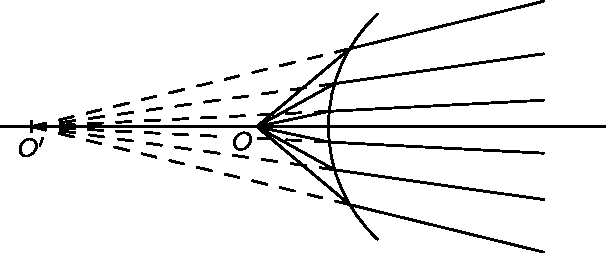
\includegraphics[width=0.7\linewidth]{fyz_fig304.pdf}
      \caption{Zdánlivý obraz
               (\cite[s.~361]{Feynman01})}
      \label{fyz:fig304}
    \end{figure}
    
    Zajímavá situace nastane, je-li \(s\) menší než \(f\) Co se stane? Když \(s<f\), \(1/s>1/f\), a 
    proto \(s'\) je záporné. Vzorec nám říká, že světlo se soustředí jen v bodě se zápornou 
    hodnotou \(s'\), ať už to znamená cokoliv. Znamená to něco velmi zajímavého a velmi užitečného. 
    Jinak řečeno, je to užitečný vzorec dokonce i tehdy, když čísla v něm jsou záporná. Situace je 
    znázorněna na obr. \ref{fyz:fig304}. Nakreslíme-li si paprsky rozcházející se z bodu \(O\), 
    budou se na povrchu lámata nesoustředí se už do jednoho bodu, neboť \(O\) je tak blízko, že už 
    jsou „za rovnoběžností“. Rozcházejí se však, jakoby vycházely z bodu \(O'\) mimo sklo. To je 
    \emph{zdánlivý obraz}, někdy nazývaný \emph{virtuální obraz}.  Obraz \(O'\) na obr. 
    \ref{fyz:fig303} se nazývá \emph{skutečný obraz}. Přichází-li světlo opravdu do nějakého bodu, 
    jde o skutečný obraz, ale zdá-li se, že světlo vychází z nějakého bodu, odlišného od původního 
    bodu, je to zdánlivý obraz. Takže vychází-li \(s'\) záporné, znamená to že \(O'\) se nachází na 
    opačné straně povrchu a vše je v pořádku.
    

    \begin{figure}[ht!] %\ref{fyz:fig305}
      \centering
      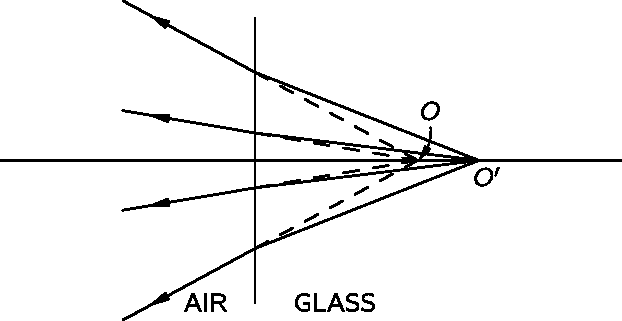
\includegraphics[width=0.7\linewidth]{fyz_fig305.pdf}
      \caption{Zdánlivý posun bodu ze zdroje \(O'\) do \(O\) při rovinném povrchu
               (\cite[s.~361]{Feynman01})}
      \label{fyz:fig305}
    \end{figure}
    
    Vezměme si zajímavý případ, kdy \(R\) je rovno nekonečnu. Pak máme \(1/s + n/s' = 0\). Jinými 
    slovy \(s' = -ns\). To znamená, že díváme-li se z hustého prostředí do řídkého a vidíme v něm 
    nějaký bod, zdá se být hlouběji o násobek \(n\). Podobně můžeme použít tutéž rovnici obráceně. 
    Díváme-li se rovinným povrchem na předmět, jenž se v hustém prostředí nachází v určité 
    vzdálenosti, bude se zdát, jakoby světlo nepřicházelo až z takové dálky (obr. 
    \ref{fyz:fig305}). Díváme-li se z hora na dno bazénu, nezdá se nám tak hluboký,jaký skutečně 
    je. Zdá se, že má jen \num{3/4} skutečné hloubky, přičemž \num{3/4} je převrácená hodnota 
    indexu lomu vody.
    
    Samozřejmě bychom mohli pokračovat a prodiskutovat problematiku kulového zrcadla. Odvození 
    rovnice pro kulové zrcadlo ponecháváme na čtenáři, ale zmíníme se, že je užitečné přijmout 
    určité konvence, týkající se vzdáleností: 
    \begin{enumerate}
      \item Předmětová vzdálenost sjekladná, nachází-li se bod \(O\) vlevo od povrchu.
      \item Obrazová vzdálenost \(s'\) je kladná, nachází-lise bod \(O\) vpravo od povrchu.
      \item Poloměr křivosti povrchuje kladný, nachází-li se střed křivosti vpravo od povrchu.
    \end{enumerate}

    Na obrázku \ref{fyz:fig303} jsou například \(s\), \(s'\) a \(R\) kladné; na obr. 
    \ref{fyz:fig304} jsou \(s\) a \(R\) kladné, ale \(s'\) je záporné. Kdybychom použili 
    \emph{konkávní povrch}, vzorec (\ref{fyz:eq360b}) by stále platil, pouze \(R\) by byla záporná 
    veličina. Při odvozování příslušného vzorce pro zrcadlo (s použitím uvedených konvencí) 
    zjistíme, že správný vzorec pro zrcadlo dostanete tak, že v rovnici (\ref{fyz:eq360b}) položíme 
    \(n = -1\) (jakoby index lomu materiálu za zrcadlem byl \num{-1})! I když odvození 
    rovnice (\ref{fyz:eq360b}) s použitím \emph{principu nejkratšího času} je snadné a elegantní, 
    tutéž rovnici lze samozřejmě odvodit pomocí Snellova zákona, máme-li na paměti, že úhly jsou 
    tak malé, že jejich siny lze nahradit příslušnými úhly.
    
    
  \section{Ohnisková vzdálenost čočky}\label{fyz:IchapXXVIIsecIII}
    Nyní uvažujme o jiné situaci, a to situaci velmi praktické. Většina čoček, které používáme, má 
    dva povrchy, nikoli pouze jeden. Jak se to projeví? Předpokládejme, že máme dva povrchy s 
    různými poloměry křivosti a prostor mezi nimi je vyplněn sklem (obr. \ref{fyz:fig306}). Chceme 
    studovat problém soustředění paprsků z bodu \(O\) do bodu \(O'\). Jak to lze provést? Odpověď 
    zní: Nejdříve použijeme vztah (\ref{fyz:eq360b}) pro první povrch a zapomeneme na ten druhý. 
    Zjistíme, že světlo, které vycházelo z \(O\), se bude sbíhat nebo rozbíhat (podle znaménka) z 
    nějakého jiného bodu, řekněme \(O'\). Nyní přejdeme k novému problému. Mezi sklema vzduchem  
    máme nový povrch, na nějž dopadají paprsky směřující do nějakého bodu \(O'\). Kde se budou 
    skutečně sbíhat? Znovu použijeme týž vztah! Zjistíme, že paprsky se sbíhají do bodu \(0"\). 
    Takto, je-li třeba, můžeme pro jít \num{75} povrchů s použitím jednoho vztahu a přecházet od 
    jednoho povrchu k druhému!
   
    \begin{figure}[ht!] %\ref{fyz:fig306}
      \centering
      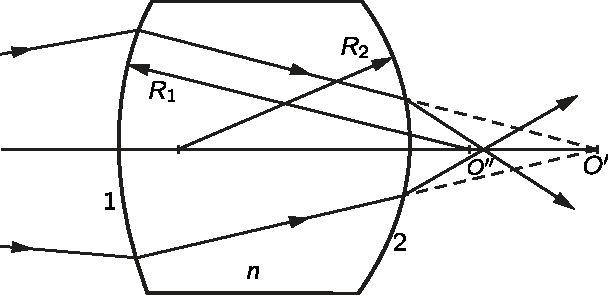
\includegraphics[width=0.7\linewidth]{fyz_fig306.pdf}
      \caption{Vznik obrazu pomocí dvoupovrchové čočky
               (\cite[s.~355]{Feynman01})}
      \label{fyz:fig306}
    \end{figure}
    
    Existují některé prvotřídní vzorce, které by nám v životě několikrát ušetřily značnou námahu 
    vynaloženou na sledování cesty světla skrz pět povrchů. Když se však setkáme s takovým 
    problémem, je jednodušší sledovat jeho cestu skrz pět povrchů, než se učit zpaměti množství 
    vzorců, které možná nikdy nebudeme potřebovat.
    
    V každém případě je princip takový, že projdeme-li jedním povrchem, najdeme polohu nového 
    ohniska, a tu vezmeme jako výchozí pro další povrch atd. Abychom to mohli skutečně provést, 
    potřebujeme zobecnit vztah (\ref{fyz:eq360b}) pro případ dvou různých indexů \(n_1\), \(n_2\) a 
    nejen pro jedno \(n\). U druhého povrchu totiž přecházíme od 	\(n\) k \(1\). místo od \(1\) k 
    \(n\) a navíc u mnoha systémů je více druhů skla s indexy \(n_1\), \(n_2\), ... atd. Není těžké 
    dokázat, že obecný tvar vztahu (\ref{fyz:eq360b}) je
    \begin{equation}  \label{fyz:eq364}
      \frac{n_1}{s} + \frac{n_2}{s'} = \frac{n_2-n_1}{R}.    
    \end{equation}
    
    Obzvlášť jednoduchý je speciální případ, kdy jsou dva povrchy velmi blízko sebe - tak blízko, 
    že můžeme zanedbat malé chyby související s tloušťkou čočky. Nakreslíme-li si čočku, jaká je na 
    obr. \ref{fyz:fig307}, můžeme si položit otázku: Jak musí být čočka zkonstruována, aby 
    soustředovala světlo z bodu \(O\) do bodu \(O'\)? Předpokládejme, že světlo dopadá přesně na 
    kraj čočky do bodu \(P\). Pak zpoždění z bodu \(O\) do \(O'\) ve srovnání s přímou cestou 
    (zanedbáme-li zatím tloušťku čočky \(T\) s indexem lomu \(n_2\)) je
    \begin{equation}  \label{fyz:eq365}
      \frac{n_1h^2}{2s} + \frac{n_1h^2}{2s'}.
    \end{equation}
    
    \begin{figure}[ht!] %\ref{fyz:fig307}
       \centering
       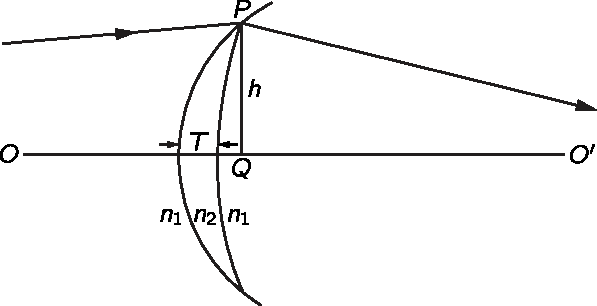
\includegraphics[width=0.7\linewidth]{fyz_fig307.pdf}
       \caption{Tenká čočka se dvěma kladnými poloměry
               (\cite[s.~355]{Feynman01})}
       \label{fyz:fig307}
    \end{figure}
    
    Aby byl čas pro přímou dráhu roven času pro dráhu \(OPO'\), musíme použít kousek skla, jehož 
    tloušťka \(T\) ve středu je taková, že zpoždění, jehož dosáhne při průchodu touto tloušťkou, 
    bude rovno zpoždění na dráze \(OPO'\). Proto tloušťka čočky v jejím středu musí být dána vztahem
    \begin{equation}  \label{fyz:eq366}
      \frac{n_1h^2}{2s} + \frac{n_1h^2}{2s'} = (n_2 - n_1)T.
    \end{equation}
    
    \(T\) můžeme vyjádřit i pomocí poloměrů křivosti \(R_1\) a \(R_2\), obou povrchů. Majíce na 
    zřeteli konvenci (3), najdeme pro \(R_1<R_2\), (konvexní čočka) vztah
      
    \begin{subequations}\label{fyz:eq367}
      \begin{align}
       T  &= \frac{h^2}{2R_1} - \frac{h^2}{2R_2}.                        \label{fyz:eq367a} \\
        \shortintertext{Proto nakonec dostáváme}
       \frac{n_1}{s} + \frac{n_1}{s'} 
          &= (n_2 - n_1)\left(\frac{1}{R_1} - \frac{1}{R_2}\right).      \label{fyz:eq367b}
      \end{align}    
    \end{subequations}
    
    Opět si všimneme, že je-li jeden z bodů v nekonečnu, druhý se bude nacházet ve vzdálenosti, 
    kterou nazveme ohnisková vzdálenost \(f\). Ohnisková vzdálenost \(f\) je dána vztahem
    \begin{equation}  \label{fyz:eq368}
      \frac{1}{f} = (n - 1)\left(\frac{1}{R_1} - \frac{1}{R_2}\right), \quad\text{kde }
      n = \frac{n_2}{n_1}.
    \end{equation}
    
    Vezmeme-li si opačný případ, kde \(s\) jde do nekonečna, vidíme, že \(s'\) se nachází v 
    ohniskové vzdálenosti \(f'\). Tentokrát jsou si ohniskové vzdálenosti rovny. (To je další, 
    speciální případ obecně platného pravidla, že poměr dvou ohniskových vzdáleností je roven 
    poměru indexů lomu dvou prostředí, v nichž se paprsky sbíhají do ohnisek. U tohoto optického 
    systému jsou počáteční a konečný index lomu stejné, takže i dvě ohniskové vzdálenosti jsou 
    stejné.)
    
    Představme si, že jsme si koupili někým zkonstruovanou čočku s určitými poloměry křivosti a s 
    určitým indexem lomu a zapomeňme na chvíli vzorec pro výpočet ohniskové vzdálenosti. Ohniskovou 
    vzdálenost bychom mohli změřit, řekněme tak, že bychom našli místo, kde se zobrazí nekonečně 
    vzdálený bod. Kdybychom už jednou znali ohniskovou vzdálenost, bylo by pro nás lepší přepsat 
    náš vzorec přímo pomocí ohniskové vzdálenosti. Dostane tvar 
    \begin{equation}  \label{fyz:eq369}
      \frac{1}{s} + \frac{1}{s'} = \frac{1}{f}
    \end{equation}
    
    Podívejme se, jak se tento vztah uplatňuje a co z něho vyplývá za různých okolností. Nejdříve 
    to, že když jedna z veličin \(s\) a \(s'\) je nekonečná, druhá je rovna \(f\). Znamená to, že 
    rovnoběžné paprsky se soustředí ve vzdálenosti \(f\) a to je vlastně definice \(f\). Další 
    zajímavostí, kterou nám říká tento vztah, je, že oba body se pohybují stejným směrem. Když se 
    jeden pohybuje směrem doprava, druhý také. Pozoruhodné je i to, že \(s\) a \(s'\) jsou si 
    rovny, rovnají-li se \(2f\). Jinými slovy zjistíme, že symetrická situace nastane, budou-li oba 
    body ve vzdálenosti \(2f\).
    
  \section{Zvětšení}\label{fyz:IchapXXVIIsecIV}
    Dosud jsme se zabývali jen zobrazováním bodů ležících na ose. Abychom pochopili vlastnosti 
    zvětšení, zabývejme se zobrazováním předmětů, jež neleží na ose, ale jsou blízko ní. Kdybychom 
    použili čočku k soustředění světla z malého vlákna do „bodu“ na stínítku, všimli bychom si, že 
    na stínítku dostáváme „obraz“ téhož vlákna, ale pouze větších nebo menších rozměrů než je 
    skutečné vlákno. To musí znamenat, že do ohniska přichází světlo z každého bodu vlákna. Abychom 
    to trochu lépe pochopili, analyzujme systém tenké čočky, schematicky znázorněný na obr. 
    \ref{fyz:fig308}. Známe tato fakta:

    \begin{figure}[ht!] %\ref{fyz:fig308}
      \centering
      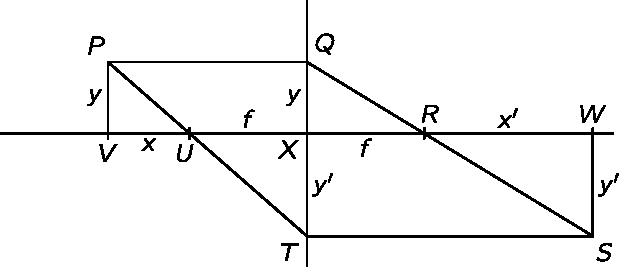
\includegraphics[width=0.7\linewidth]{fyz_fig308.pdf}
      \caption{Geometrie zobrazování pomocí tenké čočky
               (\cite[s.~355]{Feynman01})}
      \label{fyz:fig308}
    \end{figure}

    \begin{enumerate}
      \item  Kterýkoliv paprsek přicházející rovnoběžně s osou z jedné strany prochází na druhé 
             straně bodem nazvanŷm ohniskove vzdâlenosti \(f\) od čočky.
      \item  Kterýkoliv paprsek dopadající na čočku z ohniska na jedné straně vychází na druhé 
             straně rovnoběžně s osou.
    \end{enumerate}

    To je všechno, co potřebujeme ke geometrickému vyjádření vztahu (\ref{fyz:eq369}): 
    Předpokládejme, že vně jaké vzdálenosti \(x\) od ohniska máme předmět výšky \(y\). Víme, že 
    jeden z paprsků, konkrétně \(PQ\), se bude lámat tak, že bude procházet ohniskem \(R\) na druhé 
    straně. Když čočka vůbec zobrazí bod \(P\) můžeme zjistit, kde to bude, najdeme-li, kudy půjde 
    alespoň jeden další paprsek; bude to tam, kde se tyto dva paprsky opět protnou. Abychom našli 
    směr dalšího paprsku, stačí nám použít jen svůj důvtip. Víme, že rovnoběžný paprsek bude 
    procházet ohniskem - paprsek procházející ohniskem vyjde rovnoběžně s osou! Proto nakreslíme 
    paprsek \(PT\) procházející \(U\). (Ve skutečnosti budou paprsky tvořící zobrazení mnohem blíž 
    k ose než ty, které jsme si nakreslili, ale ty lze hůře nakreslit, takže budeme věřit, že 
    můžeme použít námi zobrazený paprsek.) Protože bude vycházet rovnoběžně, nakreslíme \(TS\) 
    rovnoběžně s \(XW\). Průsečík \(S\) je bod, který potřebujeme. Určí nám správnou vzdálenost i 
    správnou výšku. Výšku nazveme \(y'\) a vzdálenost od ohniska \(x'\). Nyní můžeme odvodit 
    rovnici čočky. Použitím podobných trojúhelníků \(PVU\) a \(TXU\) najdeme
    \begin{subequations}\label{fyz:eq370}
      \begin{align}
       \frac{y'}{f}  &= \frac{y}{x}.                                     \label{fyz:eq370a}  \\
        \shortintertext{Podobně z trojúhelníků \(SWR\) a \(QXR\) dostáváme}
       \frac{y'}{x'} &= \frac{y}{f}.                                     \label{fyz:eq370b}  \\
        \shortintertext{Porovnáním podílů \(\frac{y'}{y}\) z každé rovnice najdeme, že}
        \frac{y'}{y} &= \frac{x'}{f} = \frac{f}{x}.                      \label{fyz:eq370c}
      \end{align}    
    \end{subequations}
    
    Rovnice (\ref{fyz:eq370c}) je známá rovnice čočky (\emph{zobrazovací rovnice}). V ní je vše, co 
    potřebujeme o čočkách vědět: Udává nám zvětšení \(y'/y\) pomocí vzdáleností a ohniskových 
    vzdáleností. Rovněž dává do souvislosti obě vzdálenosti \(x\) a \(x'\) s \(f\)
    \begin{equation}  \label{fyz:eq371}
      xx' = f^2,
    \end{equation}
    což je vztah, s nímž se pracuje mnohem snadněji než s rovnicí (\ref{fyz:eq369}). Označíme-li 
    \(s = x + f\) a \(s' = x' + f\), uvidíme, že rovnice (\ref{fyz:eq369}) je stejná jako rovnice 
    (\ref{fyz:eq371}).
    
  \section{Složené čočky}\label{fyz:IchapXXVIIsecV}
    Bez odvozování uvedeme obecný výsledek pro řadu čoček. Jak lze analyzovat soustavu složenou z 
    několika čoček? To je snadné. Začneme nějakým předmětem a pomocí vztahu (\ref{fyz:eq371}) nebo 
    (\ref{fyz:eq369}) nebo pomocí kteréhokoliv rovnocenného vztahu nebo grafiky najdeme zobrazení 
    první čočkou. Máme tedy nějaký obraz. Pak budeme tento obraz považovat za zdroj pro další čočku 
    a ať už je její ohnisková vzdálenost jakákoliv, najdeme jí vytvořený obraz. Takto jednoduše 
    projdeme celou posloupnost čoček. To je celé umění. V principu nejde o nic nového, takže to 
    nebudeme rozebírat. Existuje však velmi zajímavý celkový výsledek působení jakékoliv řady čoček 
    na světlo, jež vzniká i končí v tomtéž prostředí, řekněme ve vzduchu. Kterýkoliv optický 
    přístroj - teleskop nebo mikroskop s jakýmkoliv množstvím čoček a zrcadel - má následující 
    vlastnost. Existují dvě roviny nazývané \emph{hlavními rovinami} soustavy (často jsou velmi 
    blízko k prvnímu povrchu první čočky a k poslednímu povrchu poslední čočky), jež mají tyto 
    vlastnosti: 
    \begin{enumerate}
      \item Když světlo dopadá rovnoběžně na soustavu z první strany, bude ven vycházet tak, že 
             se soustředí v určitém ohnisku vzdáleném od druhé hlavní roviny o ohniskovou 
             vzdálenost právě tak, jakoby soustavu tvořila tenká čočka umístěná v této rovině.
      \item Když rovnoběžné světlo přichází z druhé strany, soustředí se ve stejné vzdálenosti 
            \(f\) od první hlavní roviny, opět, jakoby tam byla umístěna tenká čočka (viz obr. 
            \ref{fyz:fig309}). 
    \end{enumerate}
    
    \begin{figure}[ht!] %\ref{fyz:fig309}
      \centering
      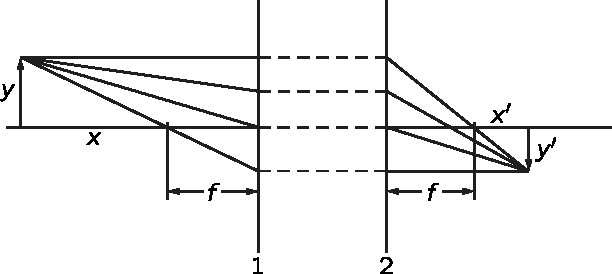
\includegraphics[width=0.7\linewidth]{fyz_fig309.pdf}
      \caption{Znázornění hlavních rovin optické soustavy
               (\cite[s.~355]{Feynman01})}
      \label{fyz:fig309}
    \end{figure}
    
    Samozřejmě, když odměříme vzdálenost \(x\) a \(x'\), \(y\) a \(y'\) jako předtím, rovnice 
    (\ref{fyz:eq371}), kterou jsme napsali pro tenkou čočku, platí zcela obecně za předpokladu, že 
    ohniskovou vzdálenost měříme od hlavních rovina ne od středu čočky. Pro tenkou čočku vychází, 
    že hlavní roviny jsou totožné. Vypadá to právě tak, jako kdybychom vzali tenkou čočku, rozřízli 
    ji podélně středem, rozdělili ji a ani si nevšimli, že je rozdělená. Každý dopadající paprsek 
    ihned vychází na vnější straně druhé roviny z téhož bodu jako dopadal na první rovinu! Hlavní 
    roviny a ohniskovou délku lze zjistit experimentálně nebo výpočtem a tím jsou určeny všechny 
    vlastnosti optické soustavy. Velmi zajímavé je, že když se takto vypořádáme s velkou složitou 
    optickou soustavou, dostaneme jednoduchý výsledek.
    
  \section{Aberace}\label{fyz:IchapXXVIIsecVI}
    Dříve než bychom se příliš nadchli tím, jak jsou čočky báječné, musíme si pospíšit dodat, že 
    jsou zde vážné nedostatky, vyplývající z toho, že jsme se omezili pouze na paraxiální paprsky, 
    tj. na paprsky blízko optické osy. U reálné čočky s konečnými rozměry se projeví 
    \textbf{aberace}. Například paprsek ležící na ose prochází ohniskem; paprsek, jenž je velmi 
    blízko osy, bude ještě stále docela dobře procházet ohniskem, ale jakmile se začneme vzdalovat, 
    paprsky se začnou odchylovat od ohniska, dejme tomu, že blíž k čočce a paprsek letící v 
    blízkosti horního okraje čočky se odchýlí od ohniska o dost velkou vzdálenost. Takže místo 
    toho, abychom získali bodový obraz, dostaneme jakousi skvrnu. Tento jev se nazývá 
    \textbf{sférická aberace}, neboť je to vlastnost sférických povrchů, jež používáme místo 
    správného tvaru. Lze ji odstranit pro jakoukoliv určitou předmětovou vzdálenost pomocí změny 
    tvaru povrchu čočky nebo případným použitím více čoček tak, že aberace od jednotlivých čoček 
    mají tendenci se navzájem vyrušit. Čočky mají i jinou vadu: Světlo různé barvy má různou 
    rychlost, a tedy různý index lomu ve skle, a proto ohnisková vzdálenost dané čočky je různá pro 
    různé barvy. Zobrazíme-li bílý bod, jeho obraz bude barevný, neboť zaostříme-li na červenou, 
    bude modrá mimo ohnisko nebo naopak. Tato vlastnost se nazývá \textbf{chromatická aberace}. 
    Existují ještě další vady. Nachází-li se předmět dost daleko od optické osy, jeho obraz 
    skutečně nelze pořádně zaostřit. Nejednodušší způsob, jak to lze ověřit, je zaostřit obraz a 
    pak vychýlit čočku, takže paprsky na ni budou dopadat pod velkým úhlem vzhledem k ose. Obraz, 
    který se vytvoří, bude obvykle velmi rozmazaný a takové místo, kde by byl ostrý, nemusí 
    existovat. Takže čočky mají více druhů vad, které se konstruktér optik snaží odstranit tím, že 
    použije mnoho čoček, aby se jejich vady navzájem vyloučily. Jak pečlivě se musíme snažit 
    vyloučit aberace? Lze vytvořit absolutně dokonalou optickou soustavu? Předpokládejme, že jsme 
    sestrojili takovou optickou soustavu, jež by měla zaostřit světlo přesně do bodu. Můžeme nyní z 
    hlediska principu nejkratšího času najít podmínku pro dokonalost soustavy? Soustava bude mít 
    nějaký vstupní otvor pro světlo. Vezmeme-li paprsek nejvzdálenější od osy, jenž může projít 
    ohniskem, jsou časy pro všechny ostatní paprsky přesně stejné (samozřejmě, je-li soustava 
    dokonalá). Nic však není dokonalé, takže otázkou je, nakolik špatný může být čas pro tento 
    paprsek, aby nestálo zato ho korigovat? Záleží to na tom, jak dokonalý chceme vytvořit obraz! 
    Předpokládejme, že obraz chceme mít tak dokonalý, jak je to jen možné. Pak máme samozřejmě 
    dojem, že to musíme zařídit tak, aby všechny paprsky měly co nejpřesněji stejné časy. Ukazuje 
    se však, že to tak není a že za určitou hranicí se pokoušíme udělat něco, co je příliš jemné, 
    neboť teorie geometrické optiky tam neplatí. 
    
    Vzpomeňme si, že princip nejkratšího času, na rozdíl od principu zachování energie nebo 
    principu zachování hybnosti, není přesně formulován. Princip nejkratšího času je jen přibližný 
    a je zajímavé, jaká může být největší dovolená chyba, aby se navenek ještě neprojevila. Odpověď 
    zní, že podařilo-li se nám dosáhnout toho, aby rozdíl časů mezi maximálním paprskem (paprskem, 
    jenž je nejhorší, nejvzdálenější) a centrálním paprskem byl menší než je perioda kmitů světla, 
    nemá smysl se pokoušet o další zdokonalování soustavy. Světlo jsou kmity s danou frekvencí, 
    která souvisí s vlnovou délkou a když jsme dosáhli toho, že rozdíl časů pro různé paprsky je 
    menší než je přibližně jedna perioda, je další námaha zbytečná.
  
  \section{Rozlišovací schopnost}\label{fyz:IchapXXVIIsecVII}
    Další zajímavou otázkou, týkající se všech optických přístrojů, jejejich rozlišovací schopnost. 
    Tato problematika je zajímavá hlavně z technického hlediska. Když konstruujeme mikroskop, 
    chceme jím vidět sledované objekty. Znamená to, že když sledujeme bakterii s tečkami na obou 
    koncích, po zvětšení chceme tyto tečky vidět. Někdo by si myslel, že stačí dosáhnout 
    dostatečného zvětšení. Vždycky můžeme přidat další čočku a zvětšovat dál a dál. Šikovností 
    konstruktérů lze vzájemně kompenzovat všechny sférické a chromatické aberace, takže není 
    důvodu, proč bychom obraz nemohli stále zvětšovat. Omezení mikroskopu nespočívají v nemožnosti 
    sestrojit čočky zvětšující více než \num{2000}krát. Mohli bychom sestrojit soustavu čoček, 
    která zvětšuje \num{10 000}krát, ale stále bychom neviděli dva blízké body kvůli omezení danému 
    geometrickou optikou, proto, že nejkratší čas není přesné kritérium.
    
    \begin{figure}[ht!] %\ref{fyz:fig310}
      \centering
      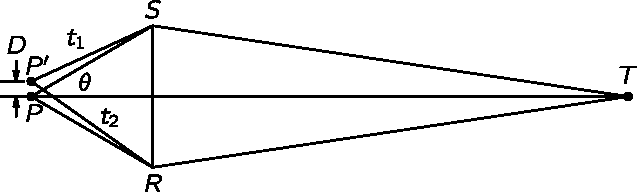
\includegraphics[width=0.7\linewidth]{fyz_fig310.pdf}
      \caption{Rozlišovací schopnost optické soustavy
               (\cite[s.~355]{Feynman01})}
      \label{fyz:fig310}
    \end{figure}
    
    Pravidlo určující, jak daleko od sebe musí být dva body, aby se jejich obrazy jevily odděleně, 
    lze velmi krásně formulovat způsobem souvisejícím s časy potřebnými pro různé paprsky. 
    Předpokládejme, že nyní aberace nebereme v úvahu a představme si, že pro určitý bod \(P\) (obr. 
    \ref{fyz:fig310}) projdou všechny paprsky od předmětu po jeho obraz \(T\) za stejný čas. (To 
    není pravda, neboť soustava není dokonalá, ale to je jiný problém.) Nyní si vezměme jiný blízký 
    bod \(P'\) o a položme si otázku, zda jeho obraz bude odlišný od \(T\). Jinými slovy, zda je 
    můžeme rozlišit. Samozřejmě, podle geometrické optiky by měly existovat dva bodové obrazy, ale 
    to, co skutečně uvidíme, může být dost rozmazané a nemusíme být schopni usoudit, že jsou tam 
    dva body. Podmínkou k tomu, aby druhý bod byl zaostřen na odlišitelně jiném místě než první, 
    je, že časy pro okrajové paprsky \(P'ST\) a \(P'RT\) na stranách čoček si pro oba body nesmí 
    být rovny, a to po drahách od obou možných předmětových bodů po daný obrazový bod. Proč? 
    Protože, kdyby si byly tyto časy rovny, je samozřejmé, že oba body by se zobrazily v témž 
    místě. Takže časy si nebudou rovny. O kolik se však musí lišit, abychom mohli říct, že se 
    nezobrazí v společném bodě a že jejich obrazy můžeme odlišit? Obecné pravidlo pro rozlišení, 
    platné pro jakoukoli optickou soustavu, je takové: Dva rozdílné bodové zdroje lze rozlišit jen 
    tehdy, když jeden zdroj se zobrazí do takového bodu, že časy potřebné pro okrajové paprsky 
    vycházející z druhého zdroje do toho bodu se v porovnání s jeho skutečným obrazovým bodem liší 
    o víc než o jednu periodu. Je třeba, aby časový rozdíl mezi horním a spodním paprskem do 
    nepravého bodu obrazu byl větší než určitá hodnota, konkrétně, aby byla přibližně rovna periodě 
    kmitů světla
    \begin{equation}\label{fyz:eq363}
       t_2 - t_1 = \frac{1}{\nu},
    \end{equation}    
    kde \(\nu\) je frekvence světla (počet kmitů za sekundu; též rychlost dělená vlnovou délkou). 
    Je-li vzdálenost mezi body rovna \(D\) a je-li úhel rozevření čočky \(\varTheta\), lze dokázat, 
    že podmínka (\ref{fyz:eq363}) je zcela rovnocenná výroku, že \(D\) musí být větší než \(\lambda 
    sin\varTheta/n\), kde \(n\) je \emph{index} v bodě \(P\) a \(\lambda\) je \emph{vlnová délka}. 
    Nejmenší věci, které tedy můžeme vidět, mají přibližně velikost vlnové délky světla. Podobný 
    vztah platí pro teleskopy; říká nám, jaký je nejmenší úhel mezi dvěma hvězdami, které lze ještě 
    rozlišit\footnote{Tento úhel je přibližně roven \(\lambda/D\), kde \(D\) je průměr čočky.}
    
  \section{Příklady a cvičení}\label{fyz:IchapXXVIIsecVIII}



 



} %tikzset
%~~~~~~~~~~~~~~~~~~~~~~~~~~~~~~~~~~~~~~~~~~~~~~~~~~~~~~~~~~~~~~~~~~~~~~~~~~~~~~~~~~~~~~~~~~~~~~~~~~
\printbibliography[title={Seznam literatury}, heading=subbibliography]
\addcontentsline{toc}{section}{Seznam literatury}